\documentclass[20pt,margin=1in,innermargin=-4.5in,blockverticalspace=-0.25in]{tikzposter}
\geometry{paperwidth=42in,paperheight=32.5in}
\usepackage[utf8]{inputenc}
\usepackage{amsmath}
\usepackage{amsfonts}
\usepackage{amsthm}
\usepackage{amssymb}
\usepackage{mathrsfs}
\usepackage{graphicx}
\usepackage{adjustbox}
\usepackage{enumitem}
\usepackage[backend=biber,style=numeric]{biblatex}
\usepackage{uomtheme}
\usepackage{multicol}

\usepackage{mwe} % for placeholder images

\addbibresource{refs.bib}


\tikzposterlatexaffectionproofoff
\usetheme{UoMTheme}
\usecolorstyle{UoMStyle}

\usepackage[scaled]{helvet}
\renewcommand\familydefault{\sfdefault} 
\usepackage[T1]{fontenc}


\title{an overview of traumatic brain injury identification and treatment approaches using data mining}
\author{Couprie Antoine,
Nguyen Thang,
Palluel Luis,
Kalavadiya Pratvi}

\institute{Université Paul Sabatier, Route de Narbonne, 31330 Toulouse, France\\
}
\titlegraphic{
\includegraphics[width=0.13\textwidth]{img/UT3+PRES_logoQ.jpg}}

% begin document
\begin{document}
\maketitle
\centering
\begin{columns}
    \column{0.32}
    \block{Problem}{
        Traumatic brain injury (TBI) is a major problem with more than 10 million people affected worldwide each year, this is also the most common neuro-logical condition in children. TBI has several recovery types which are dead, vegetative state, severe disability, moderate disability and good recovery. Permanent disability, coma and death are the usual final states of TBI patients.
    }
    \block{TBI \& Data mining}{
        TBI is the injury caused to brain by an external force. TBI refers to serious injuries of skull that alters the brain functions. TBI can be classified based on seriousness of the injury. There is no particular method which guarantees patient will recover fully.
        
        Since last few years data mining played an important role. Data mining helps clinicians to find patterns of TBI which help to treat patient so they can live normal life after suffering from this threatening disease. Data mining methods and models can either to identify the TBI in early stage or helps to recover in post treatment recovery.
        
        \begin{itemize}
            \item \textbf{TBI identification} helps to identify TBI patient.
            \item \textbf{Prediction of the post treatment recovery} helps to identify the state of the TBI patient and predicts the recovery outcome.
        \end{itemize}
        
        %Data mining methods can be of two types: predictive or descriptive. Predictive models make prediction about unknown data values by using the known values, while descriptive models identify the patterns or relationships from examined data.\cite{marcano-cedeno_artificial_2013}
    }
    
    \block{TBI Identification}{
        An overview of TBI identification base on machine learning/deep learning algorithms is illustrated in Figure \ref{fig:diagrammtbi} includes three main phases:
        \begin{itemize}
            \item \textbf{Feature extraction:} The ML/DL model tries to learn features or presentation from the image/ some MRI metrics in Table \ref{fig:diagram1}. 
            \item \textbf{Feature selection:} The extracted features combine to demographic, control together. Then these features are selected.
            \item \textbf{Classification:} These selected features are used to identify TBI patient.
        \end{itemize}
        \begin{multicols}{2}
        \begin{tikzfigure}[The MRI metrics description.]
            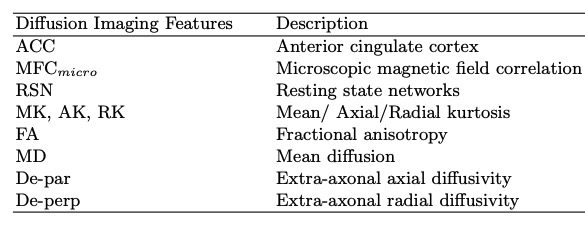
\includegraphics[width=0.9\linewidth]{img/table-metric.jpg}
            \label{fig:diagram1}
        \end{tikzfigure}
        
        \begin{tikzfigure}[An overview of TBI identification based on machine learning algorithms.]
            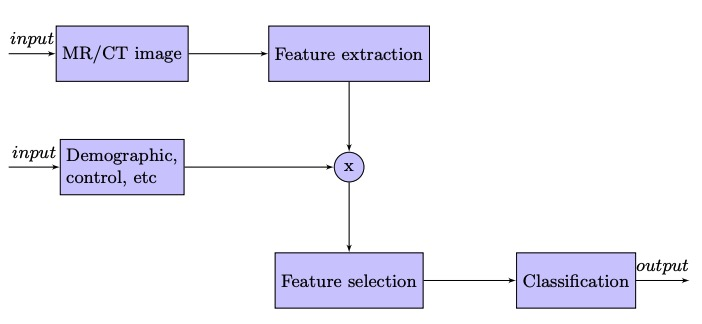
\includegraphics[width=0.9\linewidth]{img/img-tbiidentif.jpg}
            \label{fig:diagrammtbi}
        \end{tikzfigure}
        
        \end{multicols}
        \medskip
        Paper \cite{minaee_mtbi_2019}, Minaee et al use adversarial auto-encoder network for feature extraction and bag of words model for global presentation from MRI without label as shown in Figure \ref{fig:diagram2}, achieving Accurancy ($0.84$), Sensitivity ($0.86$).
        
        Vergaraa and al.~\cite{vergara_dynamic_2018} presented a dynamic functional network connectivity (dFNC) to create functional connectivity (FC) matrix from functional MR images (fMRI) and used support vector machine algorithms to classify subjects in mTBI patients with better performance, achieving (AUC)=$0.92$. 
        
        \begin{tikzfigure}[The convolutional auto-encoder.]
            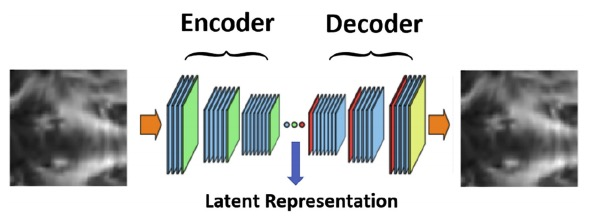
\includegraphics[width=0.6\linewidth]{img/autoencoder.jpg}
            \label{fig:diagram2}
        \end{tikzfigure}
    }
    \column{0.36}
    \block{}{
        Kamnitsas et al. \cite{kamnitsas_unsupervised_2017} proposed a useful approach for the segmentation of TBI using unsupervised domain adaption (UDA) as shown in Figure \ref{fig:diagram3} with performance close to accuracy of supervised learning.
        \begin{tikzfigure}[The multi-connected adversarial networks base-UDA.]
            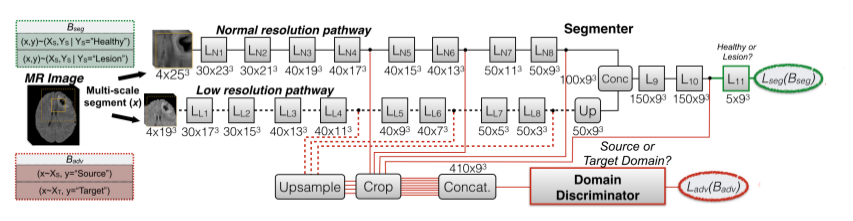
\includegraphics[width=0.7\linewidth]{img/kamnitsas_2017_pipeline.png}
            \label{fig:diagram3}
        \end{tikzfigure}
    }
    \block{Prediction of the post-treatment recovery}{
    
       	\textbf{Functional outcomes and mortality} 
        
        The objective is to predict the state of a patient with TBI, the consciousness and the mortality. 
        \begin{itemize}
            \item \textbf{State / Consciousness:} Comparing several studies, EvoLabelPred from Siddiqui and al. \cite{siddiqui_predicting_2015}  and Artificial Neural Network from Lu and al. \cite{lu_predicting_2015}  seems to have the best results for estimating and predicting the state of a patient.
\item \textbf{Mortality:} Naïve Bayes \cite{lu_predicting_2015} have one the best result in predicting the chances of dying for a TBI patient. 
        \end{itemize}
        
        \textbf{Find causalities in TBI} 
	
    The objective is to study TBI patients to have a better comprehension of this disease.
    \begin{itemize}
            \item \textbf{Increased morbidity:} Using a Topological Data Analysis, study by Nielson and al. \cite{nielson_topological_2015}  achieved several interesting conclusions as the increased number of autonomic complications for males after a TBI surgery.
    \end{itemize}
    \begin{tikzfigure}[Topological representation of the syndromic space using TDA.\cite{nielson_topological_2015}]
        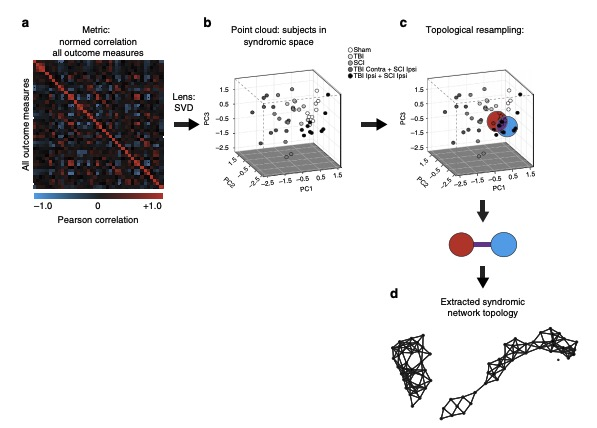
\includegraphics[width=0.6\linewidth]{img/fg1-jbvs.jpg}
        \label{fig:diagram5}
    \end{tikzfigure}
    
    \begin{itemize}
    \item \textbf{White matter:}  There are some differences in the white matter between TBI patients and healthy people. Some connections differs and TBI patients show lower fractional anisotropy in three white matter region (inferior frontal, superior frontal, and supracallosal).
    \end{itemize}
        
    
    \textbf{Emotional responses of patients}
    
    The objective is to study the emotional response of TBI patients as this is important to adapt the treatment.
    \begin{itemize}
            \item \textbf{Positive / Negative emotion:} In order to classify the emotions, the HRV is used. In the study by  F. Riganello and al. \cite{f_riganello_data-mining_2009} which consists in listening music, ONE-R classification method achieved the best results.
        \end{itemize}
        
    }

    \column{0.32}
    \block{Discussion}{
        Newer methods are applied with a variety of different and imaging modalities are used for different application. This makes comparisons of studies impracticable. Professor Duhaime speaks in favor of a standardization of the definitions and interpretation scheme in order to do a best extraction of common data element across multiple neuroimaging studies that employ different imaging techniques\cite{duhaime_common_2010}.
    }
    
    \block{Conclusion}{
        Even if it is a very serious issue, sadly, to our opinion, the number of publication is pretty poor and most of the time kind of old regarding the development of data mining. We really hope see more publications on that topic on a near future.
    }
    
    \block{Acknowledgements}{
        We would like to thank Prof. Josiane Mothe from the IRIT UMR5505 CNRS Lab, Université de Toulouse, INSPEE for her valuable comments all along the training module this document results of.
    }
    
    \block{References}{
        \vspace{-1em}
        %\bibliographystyle{splncs04}
        \begin{footnotesize}
        \printbibliography[heading=none]
        \end{footnotesize}
    }
\end{columns}
\end{document}